% 图 D.2 均匀磁化的铁磁球：球内体积 V、球外 V-bar，半径 a
\documentclass[tikz,border=5pt]{standalone}
\usetikzlibrary{arrows.meta}
\usepackage{amsmath}
\usepackage{bm}
\usepackage{fontspec}
\setmainfont{Times New Roman}
\begin{document}
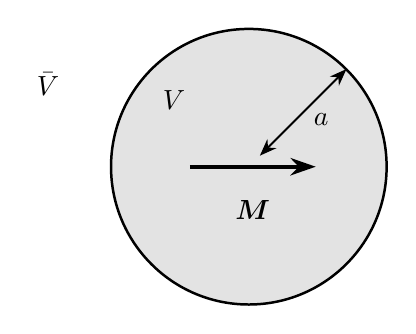
\begin{tikzpicture}[line width=0.8pt,>=Stealth]
% sphere cross-section
\draw[line width=0.9pt,fill=gray!22] (0,0) circle (1.75);
% magnetization
\draw[line width=1.5pt,-{Stealth[length=3.2mm,width=2.2mm]}] (-0.75,0) -- (0.85,0);
\node[below] at (0.05,-0.30) {$\bm{M}$};
% radius (double-headed)
\draw[<->,line width=0.7pt] (0.14,0.14) -- (1.24,1.24);
\node at (0.92,0.60) {$a$};
% volumes
\node at (-0.95,0.85) {$V$};
\node at (-2.55,1.05) {$\bar{V}$};
\end{tikzpicture}
\end{document}
